\documentclass[11pt,a4paper]{article}
\usepackage{amsmath,amssymb,amsthm}
\usepackage{graphicx}
\usepackage[margin=2.2cm]{geometry}
\usepackage{xcolor}
\usepackage{titlesec}
\usepackage{fancyhdr}
\usepackage{booktabs}
\usepackage{enumitem}
\usepackage{float}
\usepackage{hyperref}
\hypersetup{colorlinks=true,linkcolor=blue!70!black,urlcolor=blue!70!black}

\renewcommand{\topfraction}{0.9}
\renewcommand{\bottomfraction}{0.9}
\renewcommand{\textfraction}{0.07}
\renewcommand{\floatpagefraction}{0.7}
\setcounter{topnumber}{3}
\setcounter{bottomnumber}{3}
\setcounter{totalnumber}{5}

\definecolor{primary}{RGB}{0,100,60}
\definecolor{accent}{RGB}{204,102,0}

\titleformat{\section}{\Large\bfseries\color{primary}}{\thesection}{1em}{}
\titleformat{\subsection}{\large\bfseries\color{primary!80!black}}{\thesubsection}{1em}{}

\pagestyle{fancy}
\fancyhf{}
\fancyhead[L]{\small\color{primary}Essential Summary}
\fancyhead[R]{\small\color{primary}Li \& Tang (2019)}
\fancyfoot[C]{\thepage}
\renewcommand{\headrulewidth}{0.5pt}

\begin{document}

\begin{center}
{\LARGE\bfseries\color{primary}Essential Summary}\\[12pt]
{\large\bfseries A Cosine Generalized Pad\'e Approximation Method\\and Its Application in Solving Periodic Solutions\\of Strongly Nonlinear Oscillators}\\[8pt]
{\normalsize Zhenbo Li, Jiashi Tang}\\[4pt]
{\small\itshape Journal of Vibration and Shock, Vol.\ 38, No.\ 22, 159--167 (2019)\quad DOI: 10.13465/j.cnki.jvs.2019.22.023}\\[6pt]
{\small\rule{0.7\textwidth}{0.5pt}}\\[4pt]
{\small\color{accent}This is an author-prepared essential summary, not the original paper.\\Please cite the published version.}
\end{center}

\vspace{0.5em}

\section{Background and Motivation}

Classical Pad\'e approximation constructs rational functions to approximate a given power series. However, conventional Pad\'e approximants are non-periodic and typically have limits at infinity---making them unsuitable for directly approximating periodic solutions of nonlinear oscillators. While various ``quasi-Pad\'e'' methods have been proposed (e.g., using exponential functions), none had generalized the definition of Pad\'e approximation itself, nor had any directly used Pad\'e approximation to solve for periodic solutions.

The present work builds on the authors' earlier generalized Pad\'e approximation (GPA) method, which extended the numerator and denominator from polynomial functions to arbitrary continuous function series. Here, a novel \textbf{cosine-type generalized Pad\'e approximant} is constructed---whose numerator and denominator are both series of cosine functions, inherently possessing periodicity. This makes it possible for the first time to directly approximate periodic solutions of strongly nonlinear oscillators using Pad\'e approximation.

\section{Method: Two Improvement Schemes}

\subsection{Cosine Generalized Pad\'e Approximant}

The cosine-type generalized Pad\'e approximant takes the form:
\begin{equation}
x(t) = \frac{\sum_{i=0}^{m} \alpha_i \cos(i\omega t)}{\sum_{j=0}^{n} \beta_j \cos(j\omega t)}
\label{eq:approx}
\end{equation}
where $\omega$ is the generalized Pad\'e angular frequency, and $\alpha_i$, $\beta_j$ are coefficients to be determined by matching the Taylor expansion of Eq.\ \eqref{eq:approx} with the power series solution of the governing equation:
\begin{equation}
\ddot{x} + g(x) = 0, \qquad x(0) = A,\;\; \dot{x}(0) = 0
\label{eq:model}
\end{equation}
where $g(x)$ is the restoring force, which may be a polynomial, rational function, or irrational function.

\subsection{First Improvement Scheme}

In classical Pad\'e approximation, the unknown frequency $\omega$ makes direct solution difficult. The first improvement treats $\omega$ as an \textbf{active variable} with increment $\Delta\omega$, iterating from an initial guess $\omega_0$:

\begin{enumerate}[leftmargin=2em]
\item Set $\omega = \omega_0 + k\Delta\omega$ ($k$: iteration count)
\item Expand Eq.\ \eqref{eq:approx} as a Taylor series at the origin and compare with the power series solution to obtain $(m+n+1)$ equations for $\alpha_i$ and $\beta_j$
\item Evaluate the target function at $t = \pi/\omega$:
\begin{equation}
\Gamma = x(\pi/\omega) - x_1
\end{equation}
where $x_1$ is the other intersection of the orbit with the $x$-axis, determined by $\int_{x_1}^{A} g(x)\,dx = 0$
\item Terminate when $|\Gamma| < 10^{-(p+4)}$ ($p$: precision index)
\end{enumerate}

\subsection{Second Improvement Scheme (for Rational Restoring Forces)}

For symmetric rational oscillators with longer periods, the first scheme may yield unsatisfactory results. The second improvement introduces a new target function and uses piecewise description:

\begin{enumerate}[leftmargin=2em]
\item Apply the same iteration procedure with $\omega$ as the active variable
\item Define the new target function as the \textbf{derivative at half-period}:
\begin{equation}
\Gamma_2 = \left.\frac{dx}{dt}\right|_{t=\pi/\omega} - y_1
\end{equation}
where $y_1$ is the velocity of the orbit at the negative $x$-axis intersection
\item For improved accuracy, describe the solution in two segments and match them at the half-period point
\end{enumerate}

\section{Applications and Results}

The method is demonstrated on three classes of oscillators with progressively more complex restoring forces.

\subsection{Example 1: Duffing Oscillator (Polynomial Potential)}

The classic Duffing oscillator $\ddot{x} + x + x^3 = 0$ with $A = 2$. The solution obtained via the first improvement scheme (Fig.\ 1--3) shows excellent agreement with numerical integration, with absolute error below $10^{-3}$.

\begin{figure}[htbp]
\centering
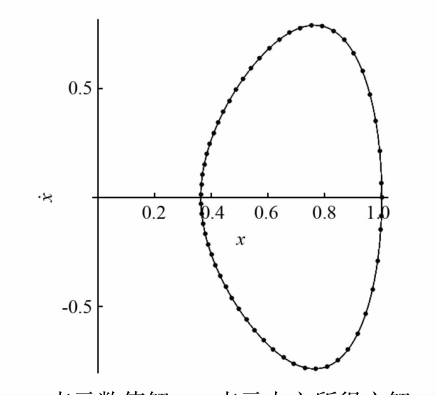
\includegraphics[width=0.85\textwidth,height=0.40\textheight,keepaspectratio]{p9-fig1.png}
\caption{Phase portrait (left), time history (center), and absolute error (right) for the Duffing oscillator with $A=2$. Solid: Runge--Kutta. Dotted: GPA.}
\end{figure}

\subsection{Example 2: Duffing-Harmonic Oscillator (Rational Potential)}

For $\ddot{x} + \frac{x + x^3}{1 + x^2} = 0$ with $A = 3$ (Fig.\ 7--9), the second improvement scheme handles the rational restoring force effectively, again with absolute error below $10^{-3}$.

\begin{figure}[htbp]
\centering
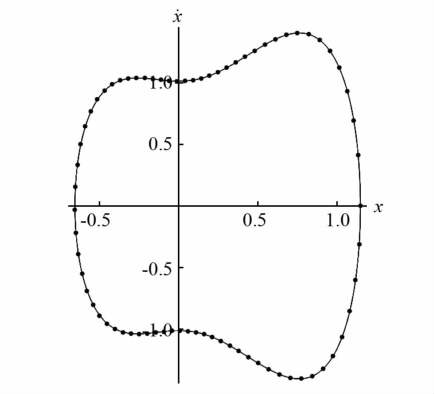
\includegraphics[width=0.85\textwidth,height=0.40\textheight,keepaspectratio]{p9-fig7.png}
\caption{Phase portrait, time history, and absolute error for the Duffing-harmonic oscillator with $A=3$.}
\end{figure}

\subsection{Example 3: SD Oscillator (Irrational Potential)}

The irrational restoring force $\ddot{x} + x\left(1 - \frac{1}{\sqrt{x^2+\alpha^2}}\right) = 0$ with $\alpha = 1$, $A = 2.5$ (Fig.\ 13). Even for this case with an irrational term arising from a geometric constraint, the cosine GPA method maintains high accuracy.

\begin{figure}[htbp]
\centering
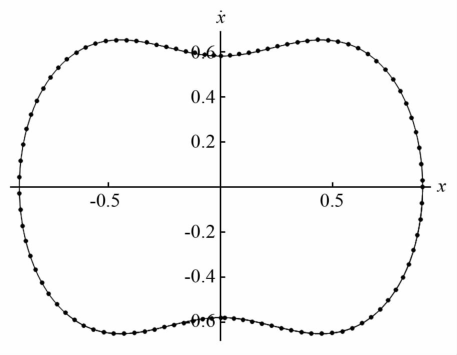
\includegraphics[width=0.80\textwidth,height=0.38\textheight,keepaspectratio]{p9-fig13.png}
\caption{Phase portrait, time history, and absolute error for the SD oscillator with $\alpha = 1$, $A = 2.5$.}
\end{figure}

\subsection{Large-Amplitude Trajectories}

Fig.\ 16 shows a \textbf{large-amplitude} trajectory for the SD oscillator with $\alpha = 0.5$, $A = 3$, and $\beta = 2$ (\emph{see original Fig.\ 16}). The method remains accurate even when the orbit spans a large region of phase space---demonstrating independence from both nonlinear coefficient magnitude and initial amplitude.

\begin{figure}[htbp]
\centering
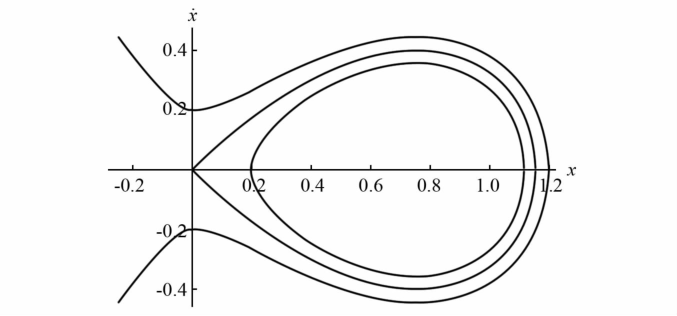
\includegraphics[width=0.85\textwidth,height=0.38\textheight,keepaspectratio]{p9-fig16.png}
\caption{Large-amplitude trajectory of the SD oscillator with $\alpha=0.5$, $A=3$, $\beta=2$.}
\end{figure}

\section{Key Findings}

\begin{enumerate}[leftmargin=2em]
\item \textbf{Cosine-type GPA enables direct periodic solution:} By constructing a generalized Pad\'e approximant with inherent periodicity, the Pad\'e framework is extended from approximating functions with limits at infinity to approximating periodic solutions---opening a new direction for Pad\'e approximation in nonlinear vibration.

\item \textbf{Two complementary improvement schemes:} The first scheme (active frequency iteration) handles polynomial potentials well; the second scheme (derivative-based target + piecewise description) extends the method to rational and irrational restoring forces with longer periods.

\item \textbf{Accuracy independent of nonlinearity strength:} Across all three classes (polynomial, rational, irrational), the absolute error consistently remains below $10^{-3}$, independent of the magnitude of nonlinear coefficients and initial amplitude.

\item \textbf{Broad applicability:} The method is demonstrated on Duffing, Duffing-harmonic, and SD oscillators---covering the three main types of restoring forces encountered in nonlinear dynamics.
\end{enumerate}

\section{Significance}

This work is the first demonstration that Pad\'e approximation can be \textbf{directly applied to periodic solution problems} through appropriate construction of the generalized approximant. It complements the authors' earlier work on using generalized Pad\'e approximation for homoclinic/heteroclinic orbits (Chin.\ Phys.\ B, 2014; 力学学报, 2013), together establishing a unified GPA framework for both periodic and non-periodic solutions of strongly nonlinear oscillators.

\vfill
\begin{center}
\small\rule{0.5\textwidth}{0.3pt}\\[4pt]
\small\color{primary} Author: Zhenbo Li (lizhenbo@usc.edu.cn)\\
\small University of South China, School of Mathematics and Physics\\
\small Hunan Key Laboratory of Mathematical Modeling and Scientific Computing
\end{center}

\end{document}
